\section{Эксперементальная часть.}

В качестве диода используется электронная лампа 2Ц2С с цилиндрическим анодом и соосным с ним катодом ($r_k \leq r_a$). Диод помещен в соленоид ,ось симметрии которого совпадает с осью симметрии электродов лампы. При пропускании через соленоид постоянного тока и подаче на анод положительного потенциала в диоде реализуются скрещенные электрические и магнитные поля, характерные для магнетрона. 

Для экспериментального определения зависимости анодного тока диода от тока соленоида служит установка, схема которой показана на рис. \ref{fig:image3}. Напряжение на электроды вакуумного диода подается от специального источника питания УИП. Накал лампы питается переменным напряжениемем $~ 2,15$ В. Разность потенциалов между анодом и катодом регулируется соответствующей ручкой источника питания. Измеряется анодное напряжение вольтметром $V_a$, находящимся на панели источника питания. Анодный ток измеряется миллиамперметром, смонтированным вместе с соленоидом на специальной плате. Соленоид $C$ питается от сети постоянного напряжения 110 В. Величина тока в соленоиде регулируется с помощью реостата $R_c$ и измеряется амперметром $I_c$. Соленоид допускает ток до 1 А.

\begin{figure}[!h]
    \centering
    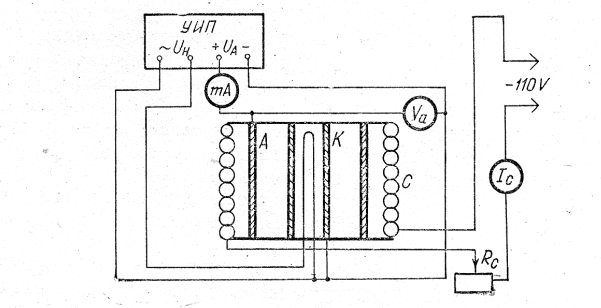
\includegraphics[width = 0.5\textwidth]{image/image3.png}
    \caption{Рис. 3}
    \label{fig:image3}
\end{figure}

Для экспериментальной установки, используемой в данной работе, имеют место следующие значения параметров:

$n_0 = 23400 \frac{1}{\text{м}}$ "--- число витков соленоида на единицу длины;

$l = 0.23$ м "--- длина соленоида;

$d = 0.1$ м "--- средний диаметр витков соленоида;

$r_a = 9.6 \cdot 10^{-3}$ м "--- радиус анода вакуумного диода.

Разбирать установку или производить какие"=либо изменения в ее схеме запрещается. На панели источника питания можно пользоваться лишь ручкой регулировки напряжения и тумблером <<сеть>>. Остальные ручки управления заблокированы и изменять их положение нельзя.

\textbf{Лабораторную работу необходимо выполнять в следующем порядке:}

\begin{enumerate}
    \item{ Включить в сеть переменного напряжения 220 В источник питания и поставить тумблер <<сеть>> в положение <<вкл>>. Через 1--2 минуты установить анодное напряжение $V_a = 150$ В. Подождать 2--3 минуты, необходимые для прогрева лампы. }
    \item{ Включить в сеть <<110 В>> с помощью специальной вилки питание соленоида. Изменяя величину тока $I_c$ в соленоиде с помощью реостата $R_c$, найти зависимость анодного тока от тока соленоида. Наиболее детальные измерения следует проводить на участке спада величины $l_a$. }
    \item{ Аналогичные измерения провести при анодных напряжениях $V_a = 200$ В и $V_a = 250$ В. Результаты измерений оформить в виде таблицы. }
    \item{ По экспериментальным данным для каждого значения анодного напряжения построить на <<миллиметровке>> зависимость $l_a = f(l_e)$. По графикам определить, как показано на рис. \ref{fig:image1}, величину критического тока в соленоиде $І_{ck}$. }
    \item{ По формуле (\ref{eq:formula4}) для каждого анодного напряжения рассчитать величины критической магнитной индукции $B_k$. }

    Преобразуя формулу (\ref{eq:formula4}), получим:
    $B_k = \mu _0 I_{ck} n_0 \frac{l}{\sqrt[2]{l^2 + d^2}} = \\ 4\pi 10^{-7}I_{ck}23400\frac{0,23}{\sqrt[2]{0,23^2 + 0,1^2}} \approx \frac{I_{ck} \cdot 23 \cdot 234 \cdot 4\pi}{10^{7} \cdot 0,250798724} = \frac{I_{ck} \cdot 21528\pi}{2507987,24} ~= 0,008583776\pi I_{ck}$

    Таким образом, для В = 160: $I_{ck} = 29,326923077$ (согласно графику)
    
    $B_k = 0,008583776 \cdot 29,326923077 \cdot 10^{-4} \cdot 3.141592653... \approx 0,0000790851\cdot$,

    для В = 200: $I_{ck} = 40,5$ (согласно графику)
    
    $B_k = 0,008583776 \cdot 40,5 \cdot 10^{-4} \cdot 3.141592653 \approx 0,0001092152468$,

    для В = 220: $I_{ck} = 48,11$ (согласно графику)
    
    $B_k = 0,008583776 \cdot 48,11 \cdot 10^{-4} \cdot 3.141592653 \approx 0,0001297369265$
    
    \item{ Вычислить для каждого анодного напряжения по формуле (\ref{eq:formula2}) величину удельного заряда электрона. Данные всех расчетов оформить в виде таблицы. Найти среднее значение удельного заряда электрона и сравнить его с табличным значением. }

    Путём элементарных преобразований формулы (\ref{eq:formula2}) получим: $\frac{e}{m} = \frac{8 V_a}{r^2_a B^2_k} = \\ = \frac{8 V_a}{(9,6 \cdot 10^{-3})^2 B^2_k} = \frac{8 V_a}{0,00009216 \cdot B^2_k} = 86805,555555556\frac{V_a}{B^2_k}$.
    Таким образом для В = 160 экспериментально: $\frac{e}{m} \approx 1,7562 \cdot 10^{11}  $,
    для В = 200 "--- : $\frac{e}{m} \approx 1,58962 \cdot 10^{11} $,
    для В = 220 "--- : $\frac{e}{m} \approx 1,472 \cdot 10^{11} $.

    Табличное значение: $1,758819 * 10^{11}$

    Среднее экспериментальное: $\frac{1,7562 + 1,58962 + 1,472}{3}10^{11} = 1,60594\cdot10^{11}$

    Отклонение от табличного: $ 1 - \frac{1,60594}{1,758819} = 0,0869214 \cdot 100\% = 8,69214\%$
\end{enumerate}

\vspace{1cm}

\textbf{Замеры \ref{tab:my_label1}:}

\begin{table}[!h]
    \centering
    \begin{tabular}{|c|c|c|c|c|c|}
         \hline
         \makecell{Замер 1\\($160B$)\\лампа\\mA} &
         \makecell{Замер 1\\($160B$)\\солиноид\\A}&
         \makecell{Замер 2\\($200B$)\\лампа\\mA} &
         \makecell{Замер 2\\($200B$)\\солиноид\\A}&
         \makecell{Замер 3\\($220B$)\\лампа\\mA} &
         \makecell{Замер 3\\($220B$)\\солиноид\\A}\\
         \hline
         $30$& $0$& $40.5$& $0$& $48.5$& $0$\\
         \hline
         $29$& $0.29$& $40.5$& $0.2$& $48$& $0.25$\\
         \hline
         $23$& $0.34$& $40.5$& $0.23$& $47.5$& $0.32$\\
         \hline
         $21$& $0.35$& $40.25$& $0.25$& $46.5$& $0.36$\\
         \hline
         $18.5$& $0.37$& $40$& $0.29$& $39$& $0.39$\\
         \hline
         $17$& $0.38$& $39$& $0.34$& $32.5$& $0.42$\\
         \hline
         $14.5$& $0.4$& $33.75$& $0.36$& $25.5$& $0.45$\\
         \hline
         $13.5$& $0.42$& $29.75$& $0.38$& $23$& $0.47$\\
         \hline
         $13$& $0.44$& $25.5$& $0.4$& $21.5$& $0.49$\\
         \hline
         $12$& $0.455$& $23.5$& $0.42$& $20$& $0.52$\\
         \hline
         $11.5$& $0.5$& $21$& $0.435$& $19.5$& $0.54$\\
         \hline
         $11$& $0.52$& $18.5$& $0.46$& $18.5$& $0.57$\\
         \hline
         $10.5$& $0.565$& $17.5$& $0.49$& $17.5$& $0.6$\\
         \hline
         $10$& $0.59$& $16.5$& $0.52$& $17$& $0.63$\\
         \hline
         & & $15.5$& $0.56$& $16$& $0.66$\\
         \hline
         & & $15$& $0.58$& $15.5$& $0.69$\\
         \hline
         & & $13.5$& $0.64$& $14.5$& $0.72$\\
         \hline
         & & $12.5$& $0.68$& $14.5$& $0.76$\\
         \hline
         & & $12$& $0.725$& & \\
         \hline
         & & $11.5$& $0.76$& & \\
         \hline
         
    \end{tabular}
    \caption{Измерения}
    \label{tab:my_label1}
\end{table}


\textbf{График замеров \ref{graph:main_graph}:}


\begin{figure}[!h]
\begin{center}
\begin{tikzpicture}
    \begin{axis}
        [
            width=\linewidth, % Scale the plot to \linewidth 
            legend pos = north east,
            xlabel=$I_c ~ mA$, % Set the labels
            ylabel=$I_a ~ A$,
            ymin = 0,
            xmin = 0,
            grid = major
        ]
        \addplot table[x=column 1,y=column 2,col sep=comma] {csvTable/table160B.csv}; 
        \addplot table[x=column 1,y=column 2,col sep=comma] {csvTable/table200B.csv};
        \addplot table[x=column 1,y=column 2,col sep=comma] {csvTable/table220B.csv};
        \legend{
            $U = 160B$,
            $U = 200B$,
            $U = 220B$,
        };
      \end{axis}
    \end{tikzpicture}
  \end{center}
\caption{График зависимости $I$ от $I_c$}
\label{graph:main_graph}
\end{figure}

\newpage

\textbf{Выводы:}

Смирнов: вычислили удельный заряд электрона "методом магнетрона" для напряжений 160, 200 и 220 В. Среднее экспериментальное значение отличается от табличного на 8,69214\%. Данная погрешность является результатом неточности в снятии показаний с вольтметра и реостата, а так же ограниченностью количества замерений.

Храмов: в качестве итога данной работы мы измерили удельный заряд электрона методом "магнетрона" для напряжений в 160, 200 и 220 вольт, заместо 150, 200 и 250 заявленных ввиду невозможности выставить данные значения без причинения потенциального вреда оборудованию. Среднее эксмпериментальное значение составило $1,60594 * 10^11$, что отклоняется от табличного лишь на 8,69214\%. Данная погрешность может быть так же объяснена, помимо компромисса для выбора напряжений, дискретным подходом для построения графика, ввиду невозможности в простых условиях получить наиболее точную зависимость $I_c$ от $I_a$.


